\documentclass[10pt]{article}

\def\Type{LessonCaelan}
\def\TypeNum{Lesson 2}
\def\TypeTitle{Introduction to Limits }
\def\Semester{Fall 2021} %Not Used 
\def\Course{MATH 1190 \& 1210}
\def\Targets{{\bf\color{RoyalBlue}L1}}

\usepackage{preambleDJ}





%%%%%%%%%%%% BEGIN DOCUMENT %%%%%%%%%%%%%%%
%%%%%%%%%%%% BEGIN DOCUMENT %%%%%%%%%%%%%%%
%%%%%%%%%%%% BEGIN DOCUMENT %%%%%%%%%%%%%%%
%%%%%%%%%%%% BEGIN DOCUMENT %%%%%%%%%%%%%%%
%%%%%%%%%%%% BEGIN DOCUMENT %%%%%%%%%%%%%%%

\begin{document}

\pagestyle{otherpages}
\thispagestyle{firstpage}
\vs{0.4}
\textbf{Intended Learning Outcomes}
After this lesson, you will be able to 

\itemC{
    \item Describe the meaning of a limit. (\target{L1})
    \item Evaluate both one-sided and two-sided limits of a function based on its graph or on a table of values and vice versa. (\target{L1})
    \item Evaluate two-sided limits by evaluating the respective one-sided limits. (\target{L1})
    \item Decide when a limit “$=\infty$” or “$=-\infty$” and interpret its meaning of such infinite limits.using a graph or a table of values. (\target{L1})
}

\vspace{-0.3cm}

\hrulefill

\vspace{0.3cm}

Problems are solved in calculus by finding ever better approximations of a desired, unknown quantity. The goal of this activity is for us to devise a mathematical tool that will empower us to improve many important approximations - ultimately, making them as accurate as needed - and to use this tool flexibly when given tables and graphs. The next $3$ exercises to decide upon some properties of such a tool before defining it.\\

%%%%%%%%%%%%%%%%%%%%%%%%

 \ie{\color{RoyalBlue}L1}The table below shows some output values of a function $f$ for input values of $x$ near $0$. 
%{\bf\color{blue} Discussion} \example{\color{RoyalBlue}L1}The table below shows some output values of a function $f$ for input values of $x$ near $0$. 
%
\begin{center}
\begin{tabular}{| c || c c c c c c |}
\hline
 $x$  & $-0.1$ & $-0.01$ & $-0.001$ &  $0.001$ & $0.01$ & $0.1$\\ 
 \hline
 $f(x)$ & $1.889$ & $1.989$  & $1.999$ & $1.999$   & $1.99$  & $1.9$\\
 \hline
\end{tabular}
\end{center}

\mpageT{.725}{.4}{
Which real value (if any) does $f(x)$ appear to approach as... 
\itemI{
\item $x$ approaches $0$ through values strictly less than $0$?$\dotfill$ \unline{.5}{}\\
\item $x$ approaches $0$ through values strictly greater than $0$?$\dotfill$ \unline{.5}{} \hs{-.13} \\
\item $x$ approaches $0$?$\dotfill$ \unline{.5}{}\\
}
}{
\centering \underline{Notation:}
}
~\\In the space below, write some rules the mathematical tool we're developing should follow based on how we made decisions in this example.

\vfill

\exercise{\color{RoyalBlue}L1} The table from the previous problem has been updated below to include the value of $f(x)$ when $x=0$.

\begin{center}
\begin{tabular}{| c || c c c c c c c |}
\hline
 $x$  & $-0.1$ & $-0.01$ & $-0.001$ & $0$ & $0.001$ & $0.01$ & $0.1$\\ 
 \hline
 $f(x)$ & $1.889$ & $1.989$  & $1.999$ & $3$ & $1.999$   & $1.99$  & $1.9$\\
 \hline
\end{tabular}
\end{center}

\mpageT{.725}{.4}{
Based on the updated table, which real value (if any) does $f(x)$ appear to approach as... 
\itemI{
\item $x$ approaches $0$ through values strictly less than $0$?$\dotfill$ \unline{.5}{}\\
\item $x$ approaches $0$ through values strictly greater than $0$?$\dotfill$ \unline{.5}{} \hs{-.13} \\
\item $x$ approaches $0$?$\dotfill$ \unline{.5}{}\\
}
}{
\centering \underline{Notation:}
}

In the space below, write some rules the mathematical tool we're developing should follow based on how we made decisions in this example. You don't have to rewrite any rules established in an earlier problem.

\vfill

\newpage
\ie{\color{RoyalBlue}L1}The table below shows some output values of the function $f$ for input values of $x$ near $2$. 
%
\begin{center}
\begin{tabular}{| c || c c c c c c |}
\hline
 $x$  & $1.9$ & $1.99$ & $1.999$ & $2.001$ & $2.01$ & $2.1$\\ 
 \hline
 $f(x)$ & $0.1$ & $0.01$  & $0.001$ & $1.002$   & $1.029$  & $1.271$\\
 \hline
\end{tabular}
\end{center}

\mpageT{.725}{.4}{
Which real value (if any) does $f(x)$ appear to approach as... 
\begin{itemize}
\item $x$ approaches $2$ through values strictly less than $2$?$\dotfill$ \unline{.5}{}\\
\item $x$ approaches $2$ through values strictly greater than $2$?$\dotfill$ \unline{.5}{} \hs{-.13} \\
\item $x$ approaches $2$?$\dotfill$ \unline{.5}{}\\
\end{itemize}
}{
\centering \underline{Notation:}
}


In the space below, write some rules the mathematical tool we're developing should follow based on how we made decisions in this example. You don't have to rewrite any rules established in an earlier problem.

\vfill

\exercise{\color{RoyalBlue}L1} The table from the previous problem has been updated below to include the value of $f(x)$ when $x=2$.

\begin{center}
\begin{tabular}{| c || c c c c c c c |}
\hline
 $x$  & $1.9$ & $1.99$ & $1.999$ & $2$ & $2.001$ & $2.01$ & $2.1$\\ 
 \hline
 $f(x)$ & $0.1$ & $0.01$  & $0.001$ & $0$ & $1.002$   & $1.029$  & $1.271$\\
 \hline
\end{tabular}
\end{center}

\mpageT{.725}{.4}{
Based on the updated table, which real value (if any) does $f(x)$ appear to approach as... 
\begin{itemize}
\item $x$ approaches $2$ through values strictly less than $2$?$\dotfill$ \unline{.5}{}\\
\item $x$ approaches $2$ through values strictly greater than $2$?$\dotfill$ \unline{.5}{} \hs{-.13} \\
\item $x$ approaches $2$?$\dotfill$ \unline{.5}{}\\
\end{itemize}
}{
\centering \underline{Notation:}
}

In the space below, write some rules the mathematical tool we're developing should follow based on how we made decisions in this example. You don't have to rewrite any rules established in an earlier problem.

\vfill

%%%%%%%%%
\newpage%
%%%%%%%%%

 \ie{\color{RoyalBlue}L1}The table below shows some output values of the function $f$ for input values of $x$ near $4$. 

\begin{center}
\begin{tabular}{| c || c c c c c c c |}
\hline
 $x$  & $3.9$ & $3.99$ & $3.999$ & $4$ & $4.001$ & $4.01$ & $4.1$\\ 
 \hline
 $f(x)$ & $4.89$ & $198.99$  & $25,147.13$ & $2$ & $-1,000,000$   & $-10,000$  & $-100$\\
 \hline
\end{tabular}
\end{center}
\mpageT{.725}{.4}{
Which real value (if any) does $f(x)$ appear to approach as... 
\begin{itemize}
\item $x$ approaches $4$ through values strictly less than $4$?$\dotfill$ \unline{.5}{}\\
\item $x$ approaches $4$ through values strictly greater than $4$?$\dotfill$\unline{.5}{}\\
\item appear to approach as $x$ approaches $4$?$\dotfill$ \unline{.5}{}\\
\end{itemize}
}{
\centering \underline{Notation:}
}
In the space below, write some rules the mathematical tool we're developing should follow based on how we made decisions in this example. You don't have to rewrite any rules established in an earlier problem.

\vfill

\exercise{\color{RoyalBlue}L1} The table from the previous problem has been updated below to correct some typos made in the first table.

\begin{center}
\begin{tabular}{| c || c c c c c c c |}
\hline
 $x$  & $3.9$ & $3.99$ & $3.999$ & $4$ & $4.001$ & $4.01$ & $4.1$\\ 
 \hline
 $f(x)$ & $4.89$ & $198.99$  & $25,147.13$ & $2$ & $1,000,000$   & $10,000$  & $100$\\
 \hline
\end{tabular}
\end{center}
\mpageT{.725}{.4}{
Which real value (if any) does $f(x)$ appear to approach as... 
\begin{itemize}
\item $x$ approaches $4$ through values strictly less than $4$?\dotfill \unline{.5}{}{.125}\\
\item $x$ approaches $4$ through values strictly greater than $4$?\dotfill \unline{.5}{}{.125}\\
\item appear to approach as $x$ approaches $4$?\dotfill \unline{.5}{}{.125}\\
\end{itemize}
}{
\centering \underline{Notation:}
}
In the space below, write some rules the mathematical tool we're developing should follow based on how we made decisions in this example. You don't have to rewrite any rules established in an earlier problem.

\vfill

%%%%%%%%%
\newpage%
%%%%%%%%%

%%%%%%%%%%%%%%%%%%%%%%%%
{\bf \blue{Notation:}} Let's give a name to the mathematical object we've been building.
\important{Limit of a Function}{
We write $\displaystyle \lim_{x\to a} f(x) = L$ and say ``the limit as $x$ approaches $a$ of $f(x)$ exists and is equal to $L$" provided we can\\ 

make $f(x)$ as close to \unline{.5}{} as we like by choosing $x$ to be as close to  \unline{.5}{} as needed \\without ever actually \unline{1.5}{} $a$.
}

\blue{\bf Matching} Let's connect informal language we've been using with more formal notation.  Which of the following phrases are connected to the math notation in the left column? In some cases, more than one phrase might be related to notation in left column.

\mpageT{.5}{.5}{
\enum{
\item $x\to a^{-}$ \\
\item $x\to a^{+}$\\
\item $x\to a$ \\
\item $\displaystyle\lim_{x\to a^{-}} f(x)$\\ \\
\item $\displaystyle\lim_{x\to a^{+}} f(x)$\\ \\
\item $\displaystyle\lim_{x\to a} f(x)$\\ \\
}
}{
\enumA{
\item $x$ approaches $a$ {\em both} through values {\em less} than $a$ {\em and} through values {\em greater} than $a$  but in both cases not  equal to $a$.\\
\item $x$ approaches $a$ through values {\em  less} than $a$ but not  equal to $a$ \\
\item $x$ approaches $a$ through values {\em greater} than $a$ but not  equal to $a$ \\
\item The trend in values of $f(x)$\\
\item The trend in values of $x$
}
}

{\bf \blue{Apply}} Now let's go back and apply this notation to Exercises A through C.\vs{.0}

{\exercise{\color{RoyalBlue}L1}} The graph of the function $f$ is shown below. Use the graph to estimate the values of the following limits. \\
\mpageTth{.325}{.325}{.325}{
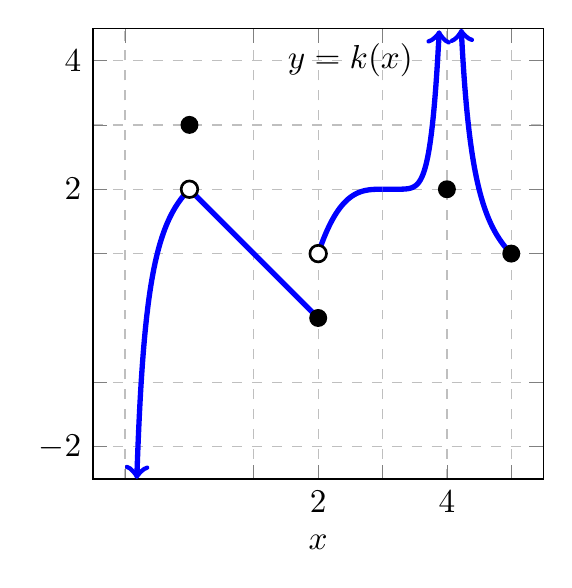
\begin{tikzpicture}[scale=1.2]
  \begin{axis}[
    xlabel={$x$},
    xtick       = {-1,1,2,3,4,5},
    xticklabels = { , ,$2$, ,$4$,},
    ytick       = {-2,-1,1,2,3,4},
    yticklabels = {$-2$, , ,$2$, ,$4$},
    samples     = 320,
    domain      = -2.5:5.5,
    restrict y to domain=-2.5:4.5,
    xmin = -1.5, xmax = 5.5,
    ymin = -2.5, ymax = 4.5,
    width = 2.5in, height = 2.5in,
    grid=both, grid style=dashed
  ]
  \node at (2.5,4) {$y=k(x)$};
  % pieces 1 & 2
  \addplot[domain=-1:0, blue, ultra thick, mark=none, <-] {3-1/(x+1)};
  \draw[blue, ultra thick] (0,2) -- (2,0);
  \filldraw[white] (0,2) circle (2.5pt);
  \draw[thick] (0,2) circle (2.5pt);
  \filldraw (0,3) circle (2.5pt);
  \filldraw (2,0) circle (2.5pt);
  % piece 3
  \addplot[domain=2:3, blue, ultra thick, mark=none] {(x-3)^3+2};
  \addplot[domain=3:4, blue, ultra thick, mark=none, ->] {6*(x-3)^7+2};
  \filldraw[white] (2,1) circle (2.5pt);
  \draw[thick] (2,1) circle (2.5pt);
  % piece 4
  \addplot[domain=4:5, blue, ultra thick, mark=none, <-] {1/(x-4)};
  %\addplot[domain=4:5, blue, ultra thick, mark=none] {-7*(x-5)^7+1};
  \filldraw (4,2) circle (2.5pt);
  \filldraw (5,1) circle (2.5pt);
\end{axis}
\end{tikzpicture}
}{
\newcommand{\spa}{.25}
\begin{enumerate}
\item[(a)] $\displaystyle\lim_{x\to0^-} f(x)=\dotfill$ \unline{.5}{}{\spa}\\
\item[(b)] $\displaystyle\lim_{x\to0^+} f(x)=\dotfill$\unline{.5}{}{\spa}\\
\item[(c)] $\displaystyle\lim_{x\to0} f(x)=\dotfill$ \unline{.5}{}{\spa}\\
\item[(d)] $\displaystyle\lim_{x\to2^-} f(x)=\dotfill$ \unline{.5}{}{\spa}\\
\item[(e)] $\displaystyle\lim_{x\to2^+} f(x)=\dotfill$ \unline{.5}{}{\spa}\\
\item[(f)] $\displaystyle\lim_{x\to2} f(x)=\dotfill$ \unline{.5}{}{\spa}\\
\end{enumerate}
}{
\newcommand{\spa}{.25}
\begin{enumerate}
\item[(g)] $\displaystyle\lim_{x\to4^-} f(x)=\dotfill$ \unline{.5}{}{\spa}\\
\item[(h)] $\displaystyle\lim_{x\to4^+} f(x)=\dotfill$ \unline{.5}{}{\spa}\\
\item[(i)] $\displaystyle\lim_{x\to4} f(x)=\dotfill$ \unline{.5}{}{\spa}\\
\item[(j)] $\displaystyle\lim_{x\to-1^+} f(x)=\dotfill$ \unline{.5}{}{\spa}\\
\item[(k)] $\displaystyle\lim_{x\to1} f(x)=\dotfill$ \unline{.5}{}{\spa}\\
\end{enumerate}
}



\newpage
\paragraph*{Note:} Problems labeled as {\bf\color{blue}Extra Practice} or {\bf\color{blue} Exam Practice} should be completed on your own for you to test your comprehension of the lesson's content, with {\bf\color{blue} Exam Practice} problems corresponding to actual exam prompts from previous semesters. The particular problem below appeared on an assessment during the Spring 2024 semester and corresponds to learning target {\bf\color{RoyalBlue}L1}. 

\

Importantly, notice that exam problems are not identical to problems seen in lessons -- but still test comprehension of the very same ideas seen in lessons. {\bf You should expect to need to adjust how you prepare for this class accordingly!}

\

Please do reach out to your instructor if you need tips on how best to prepare to be successful in this class!

\

{\bf\color{blue} Exam Practice 1.}{\reversemarginpar\marginnote{\fbox{\bf\color{RoyalBlue}L1}}} Use the seven answer choices given below to respond to the prompts that follow.  Write all correct answer choices in the blanks provided. Briefly explain your answers in the spaces provided.

\

\,\hfill
        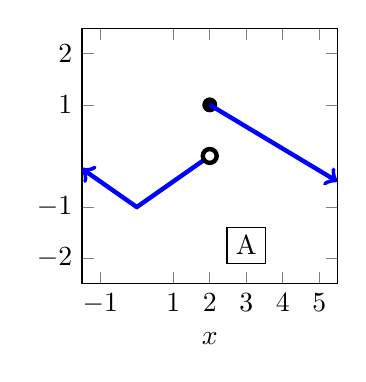
\begin{tikzpicture}[scale=1]
          \begin{axis}[
            xlabel={$x$},
            xtick       = {-1,1,2,3,4,5},
            xticklabels = {$-1$,$1$,$2$,$3$,$4$,$5$},
            ytick       = {-2,-1,1,2},
            yticklabels = {$-2$,$-1$,$1$,$2$},
            samples     = 320,
            domain      = -3:3,
            restrict y to domain=-5:5,
            xmin = -1.5, xmax = 5.5,
            ymin = -2.5, ymax = 2.5,
            width=1.9in, height=1.9in,
            %grid=both, grid style=dashed
          ]
          \node at (3,-1.75) {\fbox{A}};
          \addplot[<-,domain=-1.5:2, blue, ultra thick] {abs(x/2)-1};
          \filldraw[fill=white, ultra thick] (2,0) circle (2.5pt);
          \filldraw (2,1) circle (2.5pt);
          \draw[->, ultra thick, blue] (2,1) -- (5.5,-0.5);
        \end{axis}
        \end{tikzpicture}
\hfill
        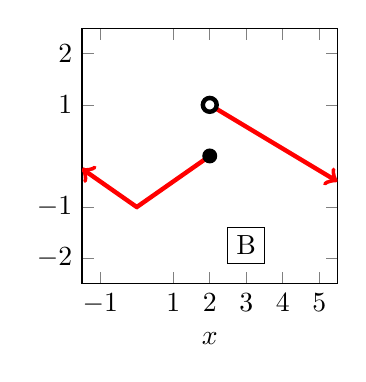
\begin{tikzpicture}[scale=1]
          \begin{axis}[
            xlabel={$x$},
            xtick       = {-1,1,2,3,4,5},
            xticklabels = {$-1$,$1$,$2$,$3$,$4$,$5$},
            ytick       = {-2,-1,1,2},
            yticklabels = {$-2$,$-1$,$1$,$2$},
            samples     = 320,
            domain      = -3:3,
            restrict y to domain=-5:5,
            xmin = -1.5, xmax = 5.5,
            ymin = -2.5, ymax = 2.5,
            width=1.9in, height=1.9in,
            %grid=both, grid style=dashed
          ]
          \node at (3,-1.75) {\fbox{B}};
          \addplot[<-,domain=-1.5:2, red, ultra thick] {abs(x/2)-1};
          \draw[->, ultra thick, red] (2,1) -- (5.5,-0.5);
          \filldraw[fill=white, ultra thick] (2,1) circle (2.5pt);
          \filldraw (2,0) circle (2.5pt);
        \end{axis}
        \end{tikzpicture}
\hfill
        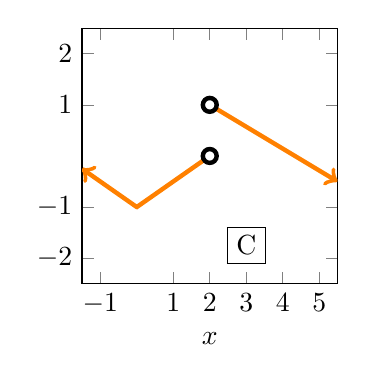
\begin{tikzpicture}[scale=1]
          \begin{axis}[
            xlabel={$x$},
            xtick       = {-1,1,2,3,4,5},
            xticklabels = {$-1$,$1$,$2$,$3$,$4$,$5$},
            ytick       = {-2,-1,1,2},
            yticklabels = {$-2$,$-1$,$1$,$2$},
            samples     = 320,
            domain      = -3:3,
            restrict y to domain=-5:5,
            xmin = -1.5, xmax = 5.5,
            ymin = -2.5, ymax = 2.5,
            width=1.9in, height=1.9in,
            %grid=both, grid style=dashed
          ]
          \node at (3,-1.75) {\fbox{C}};
          \addplot[<-,domain=-1.5:2, orange, ultra thick] {abs(x/2)-1};
          \filldraw[fill=white, ultra thick] (2,0) circle (2.5pt);
          \draw[->, ultra thick, orange] (2,1) -- (5.5,-0.5);
          \filldraw[fill=white, ultra thick] (2,1) circle (2.5pt);
        \end{axis}
        \end{tikzpicture}
\hfill\,\\
        
\,\hfill
        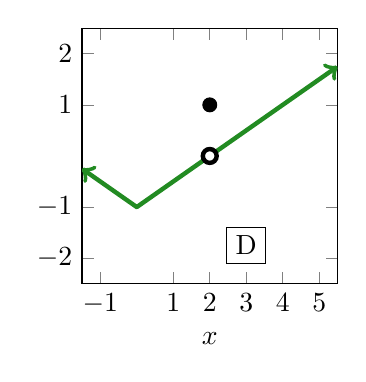
\begin{tikzpicture}[scale=1]
          \begin{axis}[
            xlabel={$x$},
            xtick       = {-1,1,2,3,4,5},
            xticklabels = {$-1$,$1$,$2$,$3$,$4$,$5$},
            ytick       = {-2,-1,1,2},
            yticklabels = {$-2$,$-1$,$1$,$2$},
            samples     = 320,
            domain      = -3:3,
            restrict y to domain=-5:5,
            xmin = -1.5, xmax = 5.5,
            ymin = -2.5, ymax = 2.5,
            width=1.9in, height=1.9in,
            %grid=both, grid style=dashed
          ]
          \node at (3,-1.75) {\fbox{D}};
          \addplot[<->,domain=-1.5:5.5, ForestGreen, ultra thick] {abs(x/2)-1};
          \filldraw[fill=white, ultra thick] (2,0) circle (2.5pt);
          \filldraw (2,1) circle (2.5pt);
        \end{axis}
        \end{tikzpicture}
\hfill
        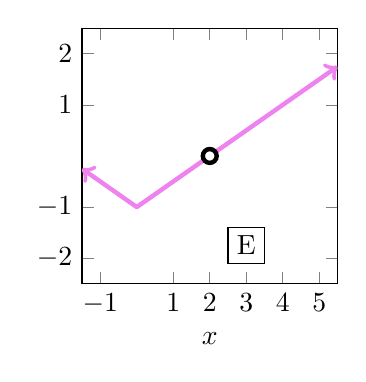
\begin{tikzpicture}[scale=1]
          \begin{axis}[
            xlabel={$x$},
            xtick       = {-1,1,2,3,4,5},
            xticklabels = {$-1$,$1$,$2$,$3$,$4$,$5$},
            ytick       = {-2,-1,1,2},
            yticklabels = {$-2$,$-1$,$1$,$2$},
            samples     = 320,
            domain      = -3:3,
            restrict y to domain=-5:5,
            xmin = -1.5, xmax = 5.5,
            ymin = -2.5, ymax = 2.5,
            width=1.9in, height=1.9in,
            %grid=both, grid style=dashed
          ]
          \node at (3,-1.75) {\fbox{E}};
          \addplot[<->,domain=-1.5:5.5, Violet, ultra thick] {abs(x/2)-1};
          \filldraw[fill=white, ultra thick] (2,0) circle (2.5pt);
          %\filldraw (2,1) circle (2.5pt);
        \end{axis}
        \end{tikzpicture}
\hfill
        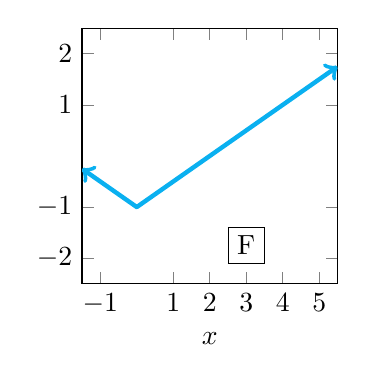
\begin{tikzpicture}[scale=1]
          \begin{axis}[
            xlabel={$x$},
            xtick       = {-1,1,2,3,4,5},
            xticklabels = {$-1$,$1$,$2$,$3$,$4$,$5$},
            ytick       = {-2,-1,1,2},
            yticklabels = {$-2$,$-1$,$1$,$2$},
            samples     = 320,
            domain      = -3:3,
            restrict y to domain=-5:5,
            xmin = -1.5, xmax = 5.5,
            ymin = -2.5, ymax = 2.5,
            width=1.9in, height=1.9in,
            %grid=both, grid style=dashed
          ]
          \node at (3,-1.75) {\fbox{F}};
          \addplot[<->,domain=-1.5:5.5, ProcessBlue, ultra thick] {abs(x/2)-1};
          %\filldraw[fill=white, ultra thick] (2,0) circle (2.5pt);
          %\filldraw (2,1) circle (2.5pt);
        \end{axis}
        \end{tikzpicture}
\hfill\,\\

\,\hfill \fbox{G} none of the other answers \hfill\,\\

\

%\,\hfill {\noindent } \hfill\,

\

\begin{enumerate}
%\item[(a)] Which of the answer choices could be the graph of a function $f$ for which $f(2)=0$? \hrulefill

%\vfill

\item[(a)] Which of the answer choices could be the graph of a function $g$ for which $\displaystyle\lim_{x\to2} g(x)$ DNE? \hfill \unline{.8}{}

\vfill

\item[(b)] Which of the answer choices could be the graph of a function $h$ for which $\displaystyle\lim_{x\to2} h(x)=1$? \hfill\unline{.8}{}

\vfill

\item[(c)] Which of the answer choices could be the graph of a function $k$ for which $\displaystyle\lim_{x\to2} k(x)=0$?\hfill \unline{.8}{}

\vfill

\end{enumerate}

\end{document}
